\chapter{Problem Description}
\label{chp:relwork}
The nature of P2P system is to help each other achieving common purpose. In this case, it is to get a particular content in the Internet. However, in the reality, this is not likely the case. It is understandable for user to be less altruistic. Although limited, an incentive system can push anyone to contribute. The distant future vision of this work is to create an \textit{European Youtube}-type of system without any central authority server. Similar to Youtube's ease-of-use, our system uses \bt~for robust streaming and without explicit file management and seeding settings. The specific goal of this research is to devise an automatic caching layer which ensures content availability for both long-lived years-old and freshly created content. This includes an automatic mechanism where every one contribute and in the same time can gain benefit to themselves. Specifically, the mechanism is an important step to reduce the needs of human intervention on contributing to improve other user's experience.

In this chapter, two problems that are the main concern of this thesis will be elaborated. First we will discuss cooperation and performance problem in peer-to-peer system, specifically \bt. The characteristics and importance of cooperation in peer-to-peer network \bt~will be reviewed. Secondly, the issue of \bt~credit and investment will be explained as the main concern of this work. It covers the importance, potential gaining, and desired effect of the possible credit investment. After specifying problems, prior works on credit mining will be reviewed. Further improvements on those work are the core of this thesis. Lastly, two research questions will be formulated.

\section{Cooperation and performance in \bt}

% social in p2p
In higher abstraction level, it is common to see P2P system, specifically in \bt, as social networking. Many social challenges, such as incentives mechanism, economic value to survive in the community, reputation identification, and user anonymity, addressed in this kind of network. All of those challenges involves peer behavior whether to help each other for the greater goods, selfishly consume all the resource without giving back, or inconsistently act between these two. It can be interpreted as maximizing their benefits and giving as little as possible. \citeauthor{2000:freeridegnutella:adar} showed that lots of P2P peers are always show self-interest and rationality \cite{2000:freeridegnutella:adar} that can be categorized as freeriding. However, \citeauthor{2005:bittorrentcooperation:andrade} showed that \bt~is indeed increased cooperation with only less than 10\% peer is uploading something. In \textit{private community}, this has gone better with higher SLR \cite{2005:bittorrentcooperation:andrade}. Even \citeauthor{2015:freeriderinbtcommunity:das} found that freerider in \bt~ does not deteriorate system performance\cite{2015:freeriderinbtcommunity:das}. All of this fact, however, does not change the fact that P2P users generally are still selfish \cite{2014:userbehaviourprivate:jia}. 

% cooperation is important in bt
In a \bt~system, cooperation between peers is crucial to keep a file available in the network. With more user provides the file, the download speed gained for other users will be increased as well. However, this needs user enthusiasm for providing the file regardless of its needs. For both public and private communities, the number of seeders becomes an issue that made a swarm unhealthy \cite{2010:pubpriv:meulpolder, 2014:sustainabilitytorrent:chen}. With freeriders join the swarm, naturally, it will reduce the overall performance. Furthermore, when freeriders become a majority, the swarm is as good as dead \cite{2000:freeridegnutella:adar}. 

% public vs private community. compare performance
% issue in both community. Imbalance.
\citeauthor{2010:pubpriv:meulpolder} measured that private communities have 3-5 times higher download speed compared to public communities \cite{2010:pubpriv:meulpolder}. This benefit makes joining private community is typically harder compared to public community. Despite has different performance, both public and private community suffer from a similar issue: ``Poor downloading experience''. It is widely known that public community generally has low SLR which directly affect the swarm performance. In the other hand, private tracker suffers from ``\textit{poor downloading motivation}'' as described by \citeauthor{2014:sustainabilitytorrent:chen}\cite{2014:sustainabilitytorrent:chen} although private community intended to solve low SLR issue. The poor downloading motivation on private tracker affect the sustainability of a swarm. The imbalance of demand and supply will harm new members of private community and gradually degrade the motivation to keep active in the community for another user \cite{2014:sustainabilitytorrent:chen}.

% the necessity to add more reputation management using cooperation. To monetize cooperation.
Peer-to-peer file sharing community, especially \bt~ can improve the user downloading experience. It does not give strain to server connection and naturally will download as fast as possible depending on file availability. However, uncooperative peer behavior and low file availability can affect a swarm's health thus reducing download experience. To complement tit-for-tat mechanism, it is necessary to implement global incentive scheme in \bt. Some researchers start by leveraging the reputation system for peers. This also supported by \citeauthor{2002:reputationtotragedy:milinski} that reputation can help solving ``tragedy of the commons'' problem \cite{2002:reputationtotragedy:milinski}. The mechanism can be centralized on decentralized. Private communities that enforce SRE is an example of centralized mechanism. The reputation of user is stored in the server while it update the data in the communication via tracker. BarterCast \cite{2009:bartercast:meulpolder} and its successor MultiChain \cite{2015:multichain:norberhuis} are the example of decentralized incentive mechanism that works on top of reputation system. 

%Several kinds of researches already provide solutions to prevent uncooperative peer behavior, all to indirectly push higher downloading throughput on downloader.
%Most of them focused their work on the incentives for peer or alteration of the currency system itself. Tribler for example, working on a MultiChain \cite{2015:multichain:norberhuis} as a secure and accountable currency in P2P system. \citeauthor{2008:givetogetvod:Mol} published free-riding resilient algorithm for Video on Demand (VoD) in P2P environment\cite{2008:givetogetvod:Mol}. \citeauthor{2015:incentivep2pgame:kang} used game theory as a formulation to incentivize peer in order to prevent free-riding behaviour\cite{2015:incentivep2pgame:kang}. They also considered mobile P2P network which only capable of low complexity mechanism. In their work, peers are awarded with different credit depend on connection type and content.
% problem: p2p social community is good if all peer is considerable, otherwise, it sucks.bittorrent pattern flashcrowd : many S/L, only at the beginning.  deteriorate afterwards. User rewarded for providing old content?

\section{The dilemma in \bt~credit investment}
\todo{high credit : benefit user. Too high (few user): bad for community, imbalance. When to donate/invest, vice versa}
In peer-to-peer system, specifically in \bt~protocol, \textit{incentive mechanism} is introduced to tackle freeriding problem \cite{2003:bittorrent:cohen}. With limited resource possessed by each peer, there is a price that need to be paid on accessing resource. The whole collection of transaction created incentive system which should be defined in order to extract user goodness in computational way.

In economic terminology, it is necessary to specify a value of the resource that can lead to the ``wealth'' of a user. In \bt~system ``credit'' can be defined in various object. For specific, private community such as DIME\footnote{\url{www.dimeadozen.org}}, \citeauthor{2012:economicbt:kash}  defined credit as \texttt{4 x upload - download} in bytes, accumulated for all the torrent served in that community \cite{2012:economicbt:kash}. \citeauthor{2015:creditmining:capota} assume the credit on his work as the difference between uploaded and downloaded bytes. \citeauthor{2014:sustainabilitytorrent:chen} mentioned another form of credit that can be earned depend on the activity, for example, seeding more torrents, seeding longer and old torrent, and seeding torrent that consumes large disk space\cite{2014:sustainabilitytorrent:chen}. In \bt, incentive system is enforced by its choking algorithm. It prefers to give the resource to the one who has the highest credit, in this case, the upload rate. In general file-sharing peer-to-peer application, user will receive credit when they upload data to others.

With credit as a token of incentive, user can ``spend'' the credit to get service from someone else. In many communities, this means that user can download more files. It is also possible that this credit may be spent to get other facilities in the community such as right to access specific content, get higher download speed, and receive social acknowledgement. Naturally, having many credit as user disposal may be advantageous \cite{2014:sustainabilitytorrent:chen}. At the point user aware of this achievement, he may want to \textit{invest} his already owned credit to get more credit.

Although high credit for user is desirable, one must be aware the effect of overwhelming credit on few users is bad for the community. Therefore, it is important to balance credit mining and community overall performance. \citeauthor{2015:sustainabilitypt:vinko} showed that both of them have conflicting interest. High few individual performance can lead to lower overall community performance \cite{2015:sustainabilitypt:vinko}. Moreover, \citeauthor{2013:survivepriv:jia} also mentioned that oversupply swarm because of overwhelming seeders may result in lower bandwidth allocation for other users \cite{2013:survivepriv:jia}. Not to mention undersupply problem that common in public community which gives very poor performance.

We define the activity of downloading with the expectation of obtaining credit to use later on as \textit{investment}. The act of seeding to help to increase the community performance graciously is called \textit{donating}. A user can \textit{prospect} which community he will invest or donate regardless of his own resource. Not all the swarm need to be seeded as we shown the drawbacks of oversupply. The prospecting and identifying swarm that needs to be seeded based on the seeder's intention (whether to invest or donate) is important. By providing proper prospecting function, users could help each other to improve the swarm quality. In good investing algorithm, users can make better use of its resource to gain credits when prospecting a swarm. 

To the best of our knowledge, there are very few works addressed credit investment in \bt. \citeauthor{2013:survivepriv:jia} mentioned how inefficient the practice of seeding for a long time to get credits. Ironically, the long time seeding is commonly practiced as it is the most trivial way to maintain credits \cite{2013:survivepriv:jia}. Three prior work has been done by \citeauthor{2015:creditmining:capota} \cite{2015:creditmining:capota, 2013:investmentcm:capota, 2014:bwmarket:capota}. This will be discussed in section \ref{section:cmprior}. 

\subsection{Gain return and performance by spending credit}
% Distinction invest vs donate.
The activity of spending credit can be categorized as three : (i) \textit{trading}, (ii) \textit{investing}, and (iii) \textit{gifting} or \textit{donating}. When a user want to spend his credit to get something, we define it as \textit{trading} or buying. This is most common case, because in credit-based community, every content has its price. \textit{Gifting} is the case when a peer consciously intend to not getting any direct, immediate, or obvious return of his credits \cite{2006:gifting:ripeanu}. The purpose of this action is usually to improve the performance of a community. Gifting can also act as a reward because a peer is satisfied with the community. Investment is the activity of spending credit with the expectation of obtaining credit to use later on. 

% helping others in p2p, improve performance
Recent work on helping other user to increase downloading performance using \bt~ has been done. \citeauthor{2014:cloudseed:leon} uses \bt~ protocol to increase user download speed and at the same time reduce datacenters load. They analyze which swarm or file to help using user bandwidth information and number of connected user\cite{2014:cloudseed:leon}. From another perspective, \citeauthor{2015:coalitionbt:zhang} introduced the \textit{coalition} between \bt~ peers. Coalition is a set of peers that cooperate each other in regards to \bt~policy to minimize download completion time. They also propose coalition-compatible choking strategy to replace the current \bt~one. This research lead to significant performance improvement within the coalition \cite{2015:coalitionbt:zhang}. Although not using \bt~protocol, in \citeyear{2009:p2phelp:he}, \citeauthor{2009:p2phelp:he} proved that helper peer also can improve the streaming capacity in P2P system\cite{2009:p2phelp:he}. \citeauthor{2016:gameauctionp2pstream:mostafavi} extend this work by introducing auction aspect for uploader to choose which user will receive the bandwidth he donate \cite{2016:gameauctionp2pstream:mostafavi}. \citeauthor{2016:gameauctionp2pstream:mostafavi} used game-theory to propose new framework in uncooperative peers with maximizing the credit gain for helpers.

% the importance of healthy swarm -> public good, prevent tragedy of the common. user is selfish, it is good to donate. Reality : they want something in return -> credit. Move the problem into investment problem. 
The ideal situation of balanced high performance and sustainability in \bt~community is desired by align supply and demand as discussed in section \ref{section:suppdemand}. By gifting and helping undersupply community adequately, the optimal situation can be achieved and tragedy of the common can be prevented \cite{2002:reputationtotragedy:milinski}. However, commonly, that is not the case. P2P user are typically selfish in economical way \cite{2014:userbehaviourprivate:jia}. \citeauthor{2009:demandsupplyres:andrade} also shows that user who contribute more to the community, actually consume a lot from it. This explains that \bt~users are not altruistic enough to seed continuously. By gifting, it will take ones resource without any return. In fact, common user wanted some return as compensation. Therefore, investment is the most feasible method to balance user and community needs.

% find low price, sell high price
In classical economic principal, the key to gain benefit is to buy low and sell high. However, this property depends on the item and the market condition. If we translate it into \bt~ economic environment, the item is the file, and the condition is the swarm. \citeauthor{2012:economicbt:kash} introduced term is \textit{resale value}. Resale value is the amount of \textit{gross} credit one will get by uploading a file. In DIME case, it is 4 times uploaded bytes. In other words, resale value is the amount of return one can expect by uploading a file. We saw this mechanism as a way to incentivize user. Because by uploading one byte, a user can get 4 credit which can be used to spend/download 4 bytes. By finding popular item and suitable swarm, the potential of investment become huge.

This phenomenon is accumulated by the existing of \textit{flashcrowd} effect. Flashcrowd effect is the sudden increase in resource demand due to various reason. Newly published torrent is one of the reasons where flashcrowd effect take place \cite{2013:swarmevolution:su}. \todo{take advantage of flashcrowd}

%\\
%Anonymous Relaying performance in Tribler \cite{2015:onionroutetribler:stokkink}\\
%Significant portion when seeding million torrents \cite{2012:milliontorrent:arvid}
%
%check swarm scrape -> multiple research -> based on dump logs

% piece population study -> http://ieeexplore.ieee.org/document/4410992/?arnumber=4410992
% related : Legout's work

% characteristics : http://www.sciencedirect.com/science/article/pii/S1389128610003622

\section{Prior Credit Mining Research}
\label{section:cmprior}
Our work is based on preliminary work by \citeauthor{2015:creditmining:capota} from 2010 till 2013 \cite{2015:creditmining:capota, 2013:investmentcm:capota, 2014:bwmarket:capota}. On the prototype they made, they implement complex method with speculative download to assess the swarms\cite{2013:investmentcm:capota}. Extending this work, they introduced \textit{helper} peer to seed low capacity swarm using libtorrent \textit{share mode}\cite{2014:bwmarket:capota}. Recently, they moved into multiple swarm approach and using public community as their research object. With swarm selection policy, they observed whether helper peer can generate high credit with less downloading\cite{2015:creditmining:capota}. \citeauthor{2015:creditmining:capota} conducted emulation and simulation in their work.

\begin{figure}[t]
	\centering
	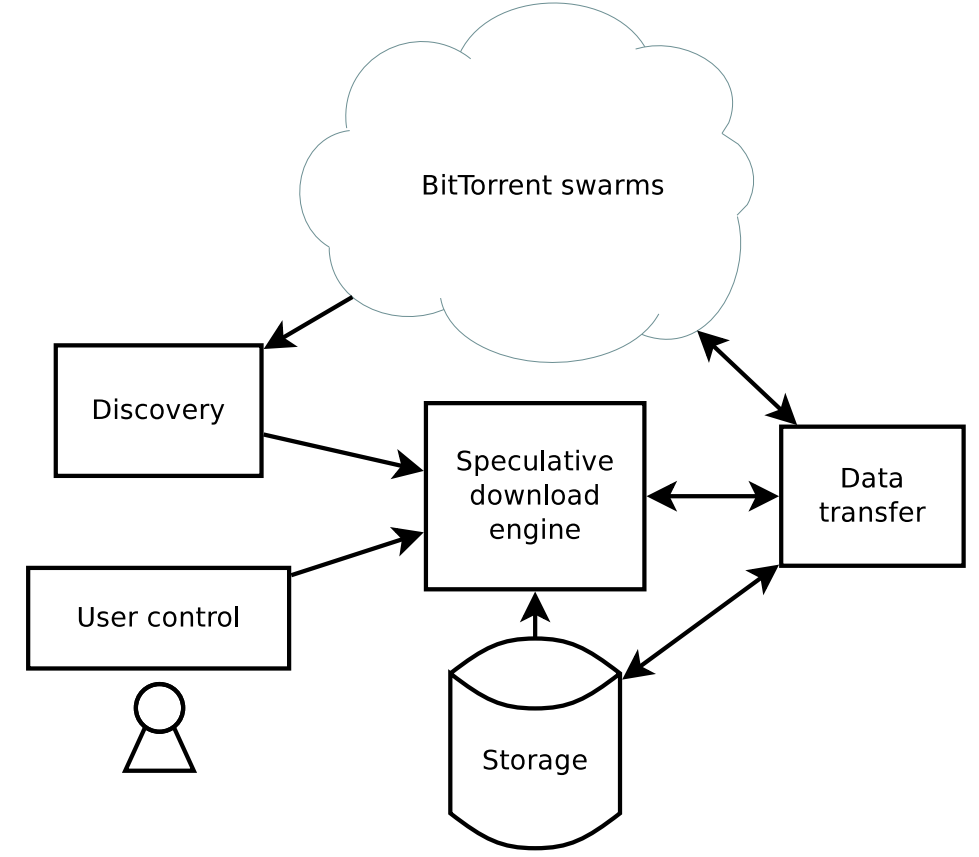
\includegraphics[width=0.7\textwidth]{pics/SDE2013.png}
	\caption{Speculative download mechanism \cite{2013:investmentcm:capota}}.
	\label{fig:sde13}
\end{figure}

In \citeyear{2013:investmentcm:capota}, \citeauthor{2013:investmentcm:capota} introduced bandwidth investing in \bt~private communities. He applied speculative download (as shown in figure \ref{fig:sde13}) on prospected swarm. This research used activity data crawled from Bitsoup\footnote{\url{https://www.bitsoup.me}} to evaluate their system. Every swarm is analyzed whether it will keep the swarm in \textit{cache} or discard it. Swarm is scored by predicting future upload speed defined in multiple regression model\cite{2013:investmentcm:capota}. One of the findings is that this algorithm depends on the size of the evaluated swarm. The more swarm need to be assessed, there is less chance the algorithm will find suitable cache to replace. This also shows the high costs and complexity of \textit{multivariate adaptive regression splines} (MARS) implemented in this system.

A year after, in \citeyear{2014:bwmarket:capota}, a research to align supply and demand in \bt~network is conducted. The idea is each peer monitor their swarms to detect whether there will be potential undersupply. If such a condition is found, one will broadcast \textit{help request} to specialized peers in order to seed this swarm. Specialized peers, called \textit{helpers}, tries to download as little as possible while upload as much as possible using \textit{libtorrent} share mode. They implement multiple helper and observe its effect to swarm with actual downloading on the other side. Their experiment result shows that using share mode in closed environment will increase download performance if the bandwidth is underutilized \cite{2014:bwmarket:capota} by shifting the bottleneck in the swarm. Moreover, \textit{libtorrent} share mode is also proven to be able to detect whether a swarm has enough capacity or not. This research also discussed flash crowd scenario. In this scenario, the existence of helper peer can lead leecher peer to reach higher download speed, especially in the early time of scenario. 

The most recent work was conducted in \citeyear{2015:creditmining:capota}\cite{2015:creditmining:capota}. \citeauthor{2015:creditmining:capota} incorporated his previous work into Credit Mining System implemented in Tribler. credit mining system able to monitor multiple swarm in one moment, and then decide which swarm this system will donate its bandwidth to. It uses simpler policy on choosing swarm compared to multivariate regression model in \cite{2013:investmentcm:capota}. As policy input, credit mining system uses torrent parameters such as seeder and leecher number obtained from tracker/DHT, creation date, length, and many others. The overview of mining process is shown in figure \ref{fig:cm15}. The experiment was conducted in live fashion on RSS \textit{etree.org}\footnote{\url{http://bt.etree.org/rss/bt\_etree\_org.rdf}} public community. They observed \textit{net upload gain} which defined as difference of uploaded bytes and downloaded bytes. Proposed policy and framework resulted in positive effect to the community.

\begin{figure}[ht]
	\centering
	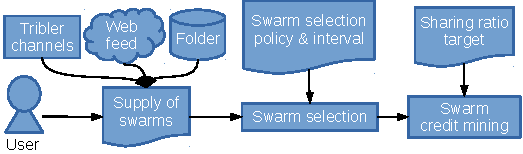
\includegraphics[width=0.8\textwidth]{pics/creditmining2015.pdf}
	\caption{The overview of credit mining process \cite{2015:creditmining:capota}}.
	\label{fig:cm15}
\end{figure}


\section{Prospecting good investment}

% emphasize on investing+prospect
Investing can not be separated by another activity called ``prospecting''. We define \textit{prospecting} as the activity to identify and measure a swarm in the hopes of getting more credit by putting a some credit as capital investment. Prospecting is the initial phase of investment, therefore, it is not needed to be comprehensive and only necessary in smaller scale. In economic perspective, not all undersupplied swarm need to be seeded, even more oversupplied swarm. Choosing a swarm to be seeded is depend on a peer available resource, intention, and investment target. In credit based community, correct investment may spark the community thus improving the performance. From user perspective, good prospecting algorithm can result a high return of the resource used from both investing and prospecting.

% crawl -> part of prospecting, knowing the swarm. 
Most researches have measured \bt~ by crawling its community pages \cite{2013:survivepriv:jia, 2005:bittorrentcooperation:andrade, 2014:userbehaviourprivate:jia, 2010:pubpriv:meulpolder, 2014:sustainabilitytorrent:chen, 2012:economicbt:kash, 2013:investmentcm:capota, 2009:demandsupplyres:andrade, 2011:interswarm:capota}. This way, they can get the data summarized by the pages. Some researches contact the tracker regularly or using its dump logs \cite{2011:yoshida:crawlbtnet, 2005:bittorrentcooperation:andrade,  2015:freeriderinbtcommunity:das, 2011:interswarm:capota}. Most of the research using logs as its dataset only use single tracker to monitor a particular torrent. Few of the research use instrumented client or directly observe the \bt~environment by understanding peer behavior \cite{2010:pubpriv:meulpolder, 2013:swarmevolution:su}. BTWorld\footnote{\url{http://btworld.nl/}} has identified four measurement techniques in \bt~\cite{2010:btworld:wojciechowski} as shown in table \ref{tbl:btmeasuremethod}. As investment need real-time data, both \textit{swarm-level} and \textit{peer-level} measurement seems to be the most compatible with prospecting method implementation. Both \textit{internet-level} and \textit{community-level} need compiled data from ISP company and community administrators, respectively \todo{any work how to measure swarm by looking at the peers?}. 

\begin{table}[ht]
	\centering
	\caption{\bt~measurement techniques \cite{2010:btworld:wojciechowski}}
	\label{tbl:btmeasuremethod}
	\begin{tabular}{|l|l|l|}
		\hline
		\rowcolor[HTML]{C0C0C0} 
		\multicolumn{1}{|c|}{\cellcolor[HTML]{C0C0C0}\textbf{Level}} & \multicolumn{1}{c|}{\cellcolor[HTML]{C0C0C0}\textbf{Advantage}} & \multicolumn{1}{c|}{\cellcolor[HTML]{C0C0C0}\textbf{Disadvantage}} \\ \hline
		Internet & Excellent coverage & ISP collaboration \\ \hline
		Community & Implementation & Peer details \\ \hline
		Swarm & Details & Context \\ \hline
		Peer & Details & Scalability \\ \hline
	\end{tabular}
\end{table}

In the following section, we will focus on the measurement technique with peer discovery. With the trackless \bt evolved in early 2008 by DHT protocol \cite{2008:dht:loewenstern}, monitoring trackers may result in inaccurate result. Moreover, the credit mining mechanism heavily rely on real-time data which can not be obtained from querying the community pages. Swarm measurement includes swarm size, peers properties, and swarm popularity. These data can be acquired both directly and indirectly by crawling peers in the swarm.

% peer discovery DHT, PEX, LSD
\subsection{Peer Discovery}
One of the integral part in \bt~protocol is peer discovery. With numerous known peers, the algorithm will have more option on which peer to unchoke. State of the swarm itself often represented by the peer belong to that swarm. It is relatively costly just to discover new peers if there are a lot of swarms monitored. \citeauthor{2012:milliontorrent:arvid} shows an example how costly the \textit{announce} request accompanied by \textit{response} payload can be in seeding a lot of torrents. Seeding 1 million torrents with announce once per every hour, which is half of the default interval, need 130 kB/s upload and 75 kB/s download bandwidth constantly \cite{2012:milliontorrent:arvid}. This value is significant for most of common Internet connection.

In \bt, there are four methods to discover new or update peer. Those are using centralized trackers, distributed hash table (DHT), peer exchange (PEX), and local service discovery (LSD). The methods will be described below. To be able fully trackerless, \textit{magnet link} extension is needed in every peer \cite{2008:magnet:hazel}. By magnet link, user can join a swarm and complete the download without using \texttt{.torrent} as its initial data. 

\subsubsection{Tracker Peer Announce}
In original design of \bt, it uses tracker to allow peer discover each other \cite{2003:bittorrent:cohen}. Tracker tends to use random and limited list of peers. Peer contact tracker periodically to expand their peer dictionary. This act of requesting peer to tracker is called \textit{announce}.	Usually, most tracker has a policy about recommended interval when to recontact for getting new peers. Violate this policy can result a particular peer blocked.	

\subsubsection{Distributed Hash Table (DHT)}
Originally, peer needs to contact tracker to fetch new peer address and file information. This makes \bt~very dependent on centralized system which vulnerable to single point of failure. In 2008, Distributed Hash Table (DHT) was proposed \cite{2008:dht:loewenstern}. Towards a ``trackerless'' \bt~system, DHT allows each peer to become a tracker. DHT stores peer contact information with defined key-space as ``node ID''. Each peer stored other peer's node ID and its address in their own routing table. A ``distance'' is measured on two node ID to define how close those two. ``Distance'' also can be measured between infohash of a torrent and node ID.

To enrich its peer dictionary, a node can compare a torrent's infohash and node ID in its routing table. If the distance under the threshold, it contacts that node to ask the information of the swarm, which includes the peer list. If contacted node do not know this torrent, it will respond with another node in its table which closest to the provided infohash. 
%\todo{expand_:DHT performance?}

\subsubsection{Peer Exchange (PEX)}
To increase the chance of getting higher downloading speed, having up to date peer is desired. This can be achieved by contacting tracker or using DHT. Reducing the interval of contacting tracker can result in getting a number of updated peer sooner, however, it will put a burden on the tracker itself. Peer Exchange (PEX )\cite{2015:PEX:the8472} is proposed to tackle this problem. PEX used list of peers that bootstrapped from another mechanism. This mechanism allows contacting known peer directly to get and give up-to-date information on swarm. Theoretically, it can keep this swarm together if trackers are down. Specification mentioned in \cite{2015:PEX:the8472} stated a restriction such as number of request per minute and number of peer added or removed in a PEX message.

\subsubsection{Local Service Directory (LSD)}
To increase the performance when downloading from a swarm, it is preferable to get the file from local network if available. Local service directory (LSD) permit this by discover peers that are in the same local network. The transfer rate is much higher compared to other type of peers. In short, LSD uses multicast-like mechanism which broadcast infohash of a torrent.

\subsection{Credit mining as investment tool}

The idea of credit mining system is to help undercapacity swarm, while at the same time to get credit for uploading data. The system try to find which swarm that might have high return by \textit{prospecting}. The investment, which relies in prospecting function, is considered with limited resources as additional requirement. Resource can be in several forms such as bandwidth, memory, or storage. Although the term ``good'' may be relative, we intend to show the efficiency of credit mining from different aspect. Therefore, we define the first research question as :

\noindent{
	\\
	\textit{How to prospect swarm and what is good investment?}\\
%	what is the properties?
	}
	
%How do we take advantage of unused bandwidth in Tribler client in non-disruptive manner?  The system address this issue by proposing activity-aware mechanism. The purpose is to get the most out of the bandwidth without disturb user of his own activity.
% What is the effect of credit mining system in live production environment?
In order to answer the question, we formulate technical challenge that need to be solved. The challenges include engineering and performance evaluation aspect. Prospecting swarm and continuously seed to gain credit may disrupt the user activity. In the other hand, it is important to take advantage of unused bandwidth. In the previous work, it is assumed that credit mining system will consume all the bandwidth. In evaluating the system, it is necessary to observe the effect of credit mining system in a whole. This can be achieved by deploying the system in live production environment. Many characteristics of swarm such as low seeder, practically dead swarm, and new published swarm will be considered. Also, the system can be improved by evaluating the properties continuously.

\section{Substituting investment cache}
In the first question, we have addressed how to gain credit as much as possible efficiently and in non-disruptive manner. However, this is not answering the limited resource available at the user disposal. Investment is a tedious activity if being done manually. Users are often forced to seed for excessively long time to maintain adequate credit \cite{2013:survivepriv:jia}. \citeauthor{2013:survivepriv:jia} also stated that this activity is commonly practiced although it is not productive. By seeding unproductively, user wastes his resources, such as bandwidth, storage capacity, and computer power. In this issue, we will specifically focus on the storage limitation. The term \textit{storage} and \textit{cache} can be used interchangeably. It points to the container used to store the swarm data as the source of investment.

To start seeding, the data must be available locally in the storage. By having many data, there are higher chance to seed many swarms as well. Eventually, it is necessary to replace obsolete investment. Several reasons to do so such as gaining less profit, unstable credit, or unreliable swarm. Downloading a swarm from nothing is costly, especially if all the content need to be downloaded. Moreover, as mentioned before, it is better to avoid both underseeded and overseeded swarm because it will affect the sustainability. By replacing old swarm by the new swarm, the balance of the ecosystem must be remained stable. The method to find which swarm that has less impact to replace by the new potential swarm is needed. Although user can control the investing process, it is desirable to do this automatically. Therefore, we define the second research question as : 

\noindent{
	\\
	\textit{When to delete a downloaded swarm and replace it with a new investment?}\\
	}
	
%What is the effect of mining in background for end-user?
Technical challenge that arise by this question is covering several aspects. It related to user behavior and intention. In the prior work, a \textit{helper} system was exist. However, either it was limited to one role per peer or all the peer in the swarm have single role. While this approach is reasonable, it is unlikely that a peer will stick to one behavior. A peer may download normally from a swarm in one time, while decide to graciously help another swarm in other time. It is also currently unknown at what point the system switches from \textit{investing} to \textit{donating}, and vice versa.